CMake开源,并且可以在许多平台上使用,还与编译器无关,从而成为构建和分发跨平台软件的强大工具。这些特性使它成为对软件极具价值的工具——可以自动化构建,以及内置的代码质量检验。

CMake由三个命令行工具组成:

\begin{itemize}
\item 
\texttt{cmake}: CMake本身,用于生成构建指令

\item 
\texttt{ctest}: CMake的测试程序,用于检测和运行测试

\item 
\texttt{cpack}: CMake的打包工具,将软件打包成方便的安装程序,如deb、RPM和自解压缩的安装程序
\end{itemize}

还有两种交互工具:

\begin{itemize}
\item 
\texttt{cmake-gui}: 配置项目的图形界面

\item 
\texttt{ccmake}: 配置CMake的交互式终端界面
\end{itemize}

\texttt{cmake-gui}可以方便地配置CMake构建,并选择要使用的编译器:

\begin{center}
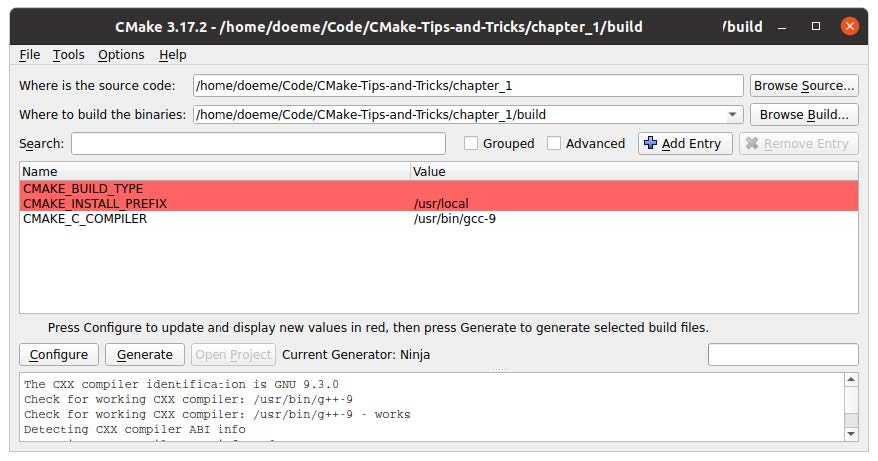
\includegraphics[width=0.8\textwidth]{content/1/chapter1/images/1.jpg}\\
图1.1  配置项目后的cmake-gui
\end{center}

若使用控制终端工作,但希望可以交互式的进行CMake配置,那么\texttt{ccmake}是不错的选择。虽然不像\texttt{cmake-gui}那样方便,但提供了相同的功能,可以通过ssh shell或类似的远程对CMake进行配置:

\begin{center}
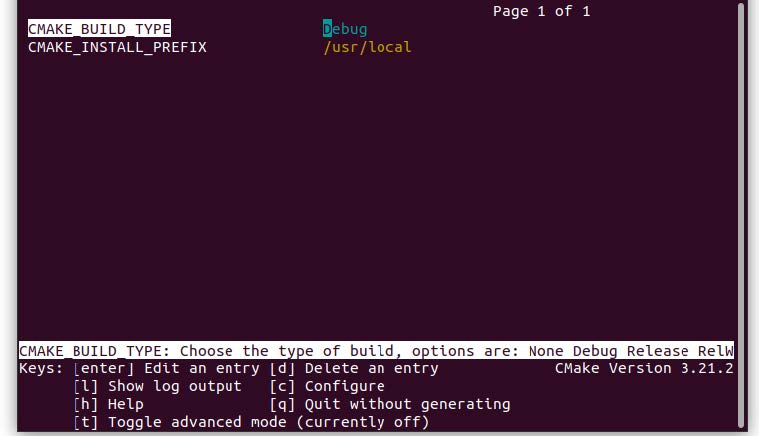
\includegraphics[width=0.8\textwidth]{content/1/chapter1/images/2.jpg}\\
图1.2  使用ccmake配置项目
\end{center}

与常规构建系统相比,CMake有很多优势。首先是跨平台方面,可以更容易地为各种编译器和平台创建构建指令,而不需要深入了解各自构建系统的细节。

然后,CMake能够发现系统库和依赖关系,这大大减轻了查找正确库的烦恼。还有就是CMake与包管理器(如Conan和vcpkg)集成得很好。

其不仅能够为多个平台构建软件,而且对测试、安装和打包的原生支持,使CMake成为构建软件的有力候选者。其能够完成从构建、测试到打包的一系列工作,对于长期维护项目有极大的帮助。

其实,CMake本身对系统的依赖很少,并且可以在命令行上运行,这使得它非常适合成为CI/CD流水中的自动化构建系统。

已经介绍了CMake可以做什么,接下来来安装CMake。






















